% This is samplepaper.tex, a sample chapter demonstrating the
% LLNCS macro package for Springer Computer Science proceedings;
% Version 2.20 of 2017/10/04
%
\documentclass[runningheads]{llncs}
%
\usepackage{graphicx}
\usepackage{float}
% Used for displaying a sample figure. If possible, figure files should
% be included in EPS format.
%
% If you use the hyperref package, please uncomment the following line
% to display URLs in blue roman font according to Springer's eBook style:
% \renewcommand\UrlFont{\color{blue}\rmfamily}

\begin{document}
%
\title{Proiect Retele de Calculatoare\\  MySSH}
%
%\titlerunning{Abbreviated paper title}
% If the paper title is too long for the running head, you can set
% an abbreviated paper title here
%
\author{Andrei-Ioan Ianău \orcidID{0000-0002-0826-1809}}

% First names are abbreviated in the running head.
% If there are more than two authors, 'et al.' is used.
%
\institute{Universitatea "Alexandru Ioan Cuza", Iași, Iași, România \\
\email{secretariat@info.uaic.ro} \\
\url{ http://www.info.uaic.ro} }
%
\maketitle              % typeset the header of the contribution
%
\begin{abstract}
Acest document descrie functionalitatea a unei aplicatii de tip "clienti-server" ce deserveste ca scop executarea de catre server a unor comenzi primite de la un client. Comunicarea va fi efectuata prin diferite metode cum ar fi sockets, pipes si fisiere fifo.


\keywords{Retele  \and Sockets \and Client-Server.}
\end{abstract}

\section{Tehnologiile utilizate}

Pentru aplicatia pe care dorim sa o realizam, vom folosi protocolul TCP. Acesta este cel mai de dorit deoarece ne permite siguranta transmiterii datelor la client si la server. Mai ales daca vom folosi encriptare, este de ajutor daca toate datele sunt transmise, astfel decriptarea sa se poata realiza.

Ce este TCP/IP?
 Spus în termeni simpli, TCP/IP este numele unei familii de protocoale de reţea.
Protocoalele sunt seturi de reguli pe care toate companiile si toate produsele software
trebuie sǎ le respecte, pentru ca produsele lor sǎ fie compatibile între ele. Un protocol
defineşte felul cum programele comunicǎ între ele. Un protocol de asemenea defineşte
felul cum fiecare parte a pachetului are grijǎ de transferal de informaţie.
 În esenţǎ, un protocol este un set scris de directive care defineşte felul în care
douǎ aplicaţii sau maşini pot comunica între ele, fiecare conformându-se cu aceleaşi
standarde. TCP/IP nu este restricţionat doar la Internet. Este protocolul de reţea cel mai
larg folosit în lume, folosit pentru reţele mari, cât si pentru reţele mici.
 TCP/IP vine de la Protocolul de Control al Transmisiei/Internet Protocol, care
sunt de fapt douǎ protocoale separate. Contrar a ce gândesc unii oameni, termenul
TCP/IP se referǎ la o întreagǎ familie de protocoale înrudite, toate proiectate pentru a
transfera informaţii prin intermediul reţelei. TCP/IP este proiectat pentru a fi componenta
software a unei reţele. Toate pǎrţile protocolului TCP/IP au anumite sarcini, cum ar fi
trimiterea de scrisori elecronice, transferal de fişiere, livrarea de servicii de logare la
distanţǎ, dirijarea de mesaje, sau manipularea cǎderilor de reţea.
 Serviciile care intrǎ in protocolul TCP/IP şi funcţiile lor pot fi grupate dupǎ
scopul lor. Protocoalele de transport controleazǎ mişcarea datelor între 2 maşini si
include urmǎtoarele:
- TCP (Transmision Control Protocol) Un serviciu bazat pe conexiuni,
însemnând cǎ maşinile care trimit şi cele care primesc sunt conectate şi
comunicǎ una cu cealaltǎ tot timpul.
- UDP (User Datagram Protocol) Un serviciu fǎrǎ conexiuni, însemnând cǎ
datele sunt trimise fǎrǎ ca maşinile care trimit şi care primesc sǎ aibǎ contact
unele cu celelalte. Este ca si cum am trimite o scrisoare prin poşta normalǎ, la
o anumitǎ adresǎ, neavând cum sǎ ştim dacǎ scrisoarea ajunge sau nu la acea
adresǎ.

TCP/IP, Internet-ul şi arhitectura stratificată
 Internet-ul nu este o singurǎ reţea, ci mai degrabǎ o colecţie de multe reţele care
comunicǎ între ele rpin protocolul TCP/IP. TCP/IP şi Internetul sunt aşa de strâns legate
încât arhitectura TCP/IP este adesea denumitǎ şi arhitecturǎ Internet. Aproape de la
începuturile internetului ca ARPAnet, a devenit evident cǎ protocoalele existente nu
puteau sǎ se descurce cu volumul foare mare al traficului pe care reţeaua trebuia sa-l
suporte, astfel un proiect a fost inieaua trebuia sa-l suporte, astfel un proiect a fost iniţiat
pentru a dezvolta noi protocoale.
 Protocoalele TCP/IP au fost propuse in anul 1973 şi au condus la o versiune
standardizatǎ, apǎrutǎ in 1982. Una dintre paginile de cercetare pentru software-ul de
reţea a fost la universitatea din Berkeley, California. Aceasta a fost centrul de devoltare
pentru sistemul de operare UNIX de-a lungul mai multor ani; cercetarea fǎcutǎ acolo a
ajutat la rafinarea protocolului TCP/IP. În 1983, universitatea a emis o versiune a UNIXului care avea incorporate protocolul TCP/IP. Protocolul a devenit foarte popular
deoarece UNIX a era folosit la scarǎ largǎ, mai cǎ din ce în ce mai multe site-uri se
conectau la ARPAnet.
 Când TCP/IP a fost proiectat, toate serviciile care trebuiau livrate au fost luate în
considerare. Cea mai bunǎ abordare pentru a implementa toate serviciile a fost cea de a
divide serviciile diferite în categorii, cum ar fi serviciile end-user (transfer de fisiere si
logare la distanţǎ), serviciile de transport (modul în care datele sunt trimise în mod
invizibil utilizatorului) şi serviciile de reţea (modul în care informaţia este împachetatǎ în
vederea trasferului). A fost dezvoltatǎ o arhitectura stratificatǎ, care izoleazǎ fiecare set
de servicii.
 O abordare stratificatǎ în rpoiectarea software-ului cere mai multǎ muncǎ initial,
dar are mai multe beneficii importante. Mai întâi, deoarece fiecare strat este independent
de celelalte, schimbǎrile la un anumit serviciu nu provoacǎ probleme cu celelalte servicii.
Pe mǎsurǎ ce noi servicii sunt dezvoltate, acestea pot fi adǎugate fǎrǎ a schimba celelalte
pǎrţi ale sistemului software. Cel mai important, stratificarea face posibil ca un set de
programe mici şi eficiente sǎ fie dezvoltate pentru scopuri specifice, fiecare fiind
independent de celelalte.
 O conditie necesarǎ pentru a permite ca arhitectura stratificatǎ sǎ funcţioneze
corespunzǎtor este cǎ fiecare strat trebuie sǎ ştie ceea ce vine de la stratul de deasupra sau
de dedesubt. Poate ca stratul sǎ nu fie interesat de conţinutul mesajului, dar trebuie sǎ ştie
ce sǎ facǎ cu el. De exemplu, dacǎ trimiteţi un e-mail, scrieţi mesaje şi comandaţi stratul
aplicaţiei sǎ transmitǎ mesajul cǎtre destinaţie. Fiecare strat se ocupǎ de mesajul e-mail,
dar nu-l intereseazǎ conţinutul mesajului.
 Pentru a simplifica aceastǎ sarcinǎ, fiecare strat adaugǎ un bloc de date în faţa şi
în spatele mesajului, ceea ce indicǎ stratul care este implicat, precum si un set de biţi
reprezentând informaţiile adǎugate de alte strate, informaţii de care maşinile care primesc 
mesajul cum trebuie. Informaţia din mesaj este ignoratǎ. Fiecare strat face propria
“încapsulare”,în sensul cǎ fiecare strat adaugǎ o capsulǎ de informaţii în jurul informaţiei
iniţiale, constituind blocuri de inceput şi sfârşit. Aceasta se materializeazǎ în câteva seturi
de header-e şi trailer-e pâna când mesajul ajunge în reţea. \cite{ref_tcp1}



\section{Arhitectura aplicatiei}
\subsection{Organizarea fisierelor}
Vom avea urmatoarele fisiere:\\
* client.c -- va contine codul ce reprezinta implementarea aplicatiei din partea clientului.  \\
* server.c  -- va contine codul ce reprezinta implementarea aplicatiei din partea serverului.  \\
README  -- un fisier ce contine scurte instructiuni pentru utilizarea aplicatiei.\\
primes.pr  -- fisier ce contine un numar mare de numere prime, ce vor fi folosite in crearea cheilor de criptare\\
users.txt -- fisier ce contine utilizatorii si parolele lor\\
run.sh  -- fisier de foloseste la testarea aplicatiei\\
Makefile    -- fisier de foloseste la dezvoltarea aplicatiei\\
constants.h  -- contine defines ce sunt folosite in intreaga aplicatie.\\
macros.h  --  contine macros ce sunt folosite in intreaga aplicatie\\
rsa.c  --  contine codul pentru criptarea de tip rsa.\\
rsa.h   --  contine declarile functiilor ce ajuta la criptare.\\
sha256.c  -- contine codul functiilor cu care se poate face hash.\\
sha256.h  -- contine declararile functiilor cu care se poate face hash.\\
utilities.c  -- contine codul functiilor ce se reutilizeaza atat la client cat si la server.\\
utilities.h -- contine declararea functiilor ce se reutilizeaza atat la client cat si la server.\\


\subsection{Flowchart}
% poza cu flowchart.

\begin{figure}[H]
  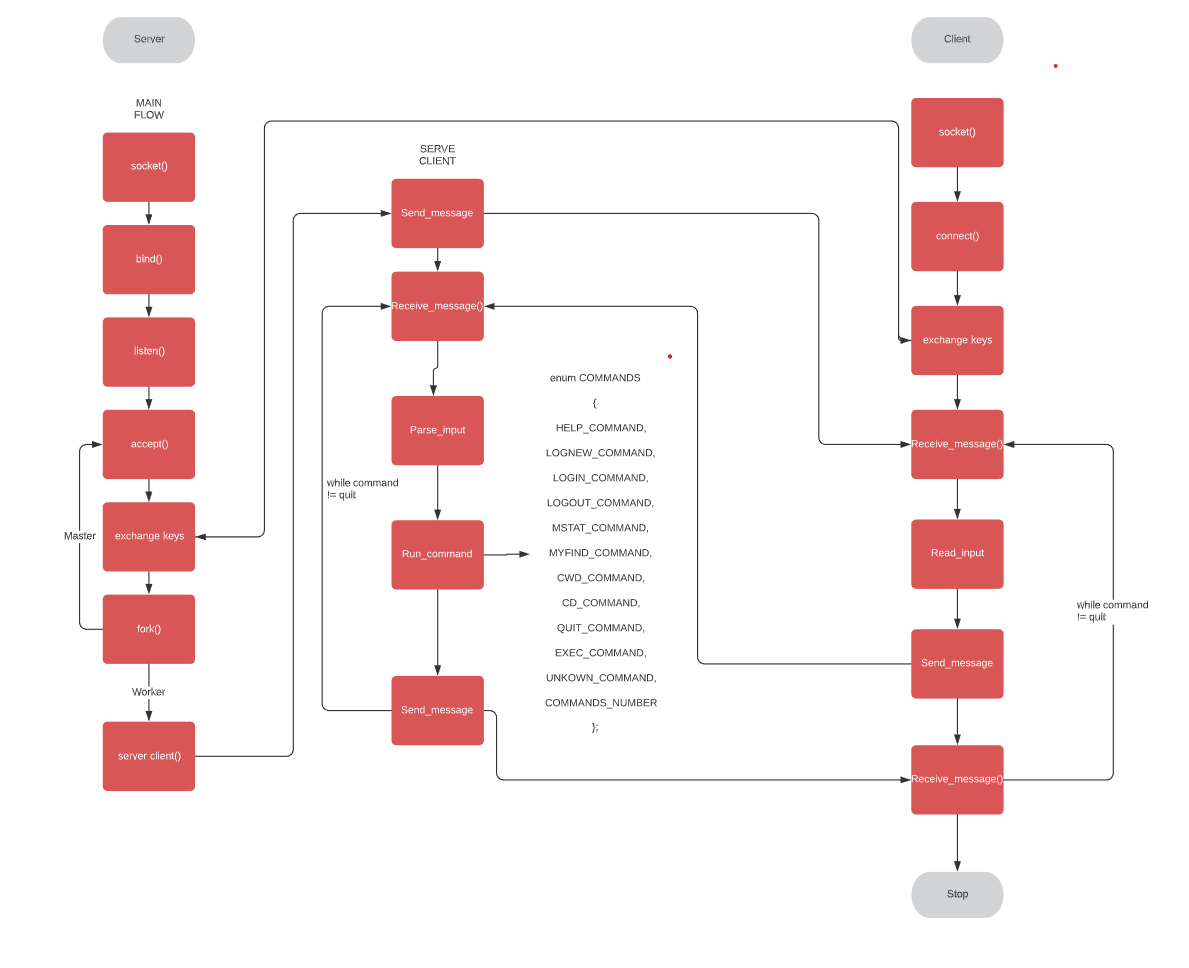
\includegraphics[width=\linewidth]{flow.png}
  \caption{Arhitectura.}
  \label{fig:flow}
\end{figure}


\subsection{Scenariu de utilizare}

Utilizatorul intra in aplicatie. I se spune ca trebuie sa se autentifice pentru a face orice alta operatie. Isi introduce credentialele. Daca nu a introdus credentialele bune, i se arata un mesaj corespunzator de eroare, altfel el este marcat ca autentificat. Acesta ruleaza comanda $exec$ $ls$ si i se va afisa rezultatul produs de catre server. Acesta poate sa inchida conexiunea prin $quit$.

\section{Detalii de implementare}

\subsection{Criptarea/Decriptarea}

Criptarea si decriptarea se fac la nivelul functiei de transmitere/primire a mesajului.
Am folosit algoritmul de criptare RSA. 
În criptografie, RSA este un algoritm criptografic cu chei publice, primul algoritm utilizat atât pentru criptare, cât și pentru semnătura electronică. Algoritmul a fost dezvoltat în 1977 și publicat în 1978 de Ron Rivest, Adi Shamir și Leonard Adleman la MIT și își trage numele de la inițialele numelor celor trei autori. \cite{ref_rsa}

Puterea sa criptografică se bazează pe dificultatea problemei factorizării numerelor întregi, problemă la care se reduce criptanaliza RSA și pentru care toți algoritmii de rezolvare cunoscuți au complexitate exponențială. Există însă câteva metode de criptanaliză care ocolesc factorizarea efectivă, exploatând maniere eronate de implementare efectivă a schemei de criptare.

\subsection{ Extinderea usoara a aplicatiei}
Un lucru care permite modularizarea si extinderea acestei aplicatii este modul in care este realizat serverul.
\begin{figure}[H]
  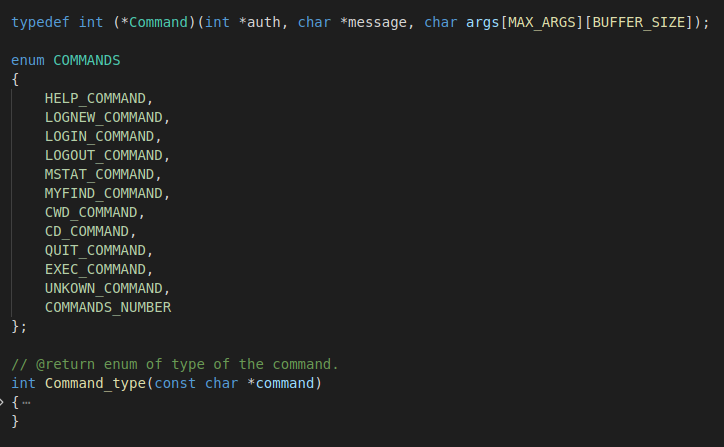
\includegraphics[width=\linewidth]{command.png}
  \caption{Modularizare.}
  \label{fig:Modularizare}
\end{figure}

Folosind astfel o modalitate de extindere a functionalitatii, vom putea apela $command[command\_type](args);$


\subsection{ Inserarea unui utilizator nou } 

\begin{figure}[H]
  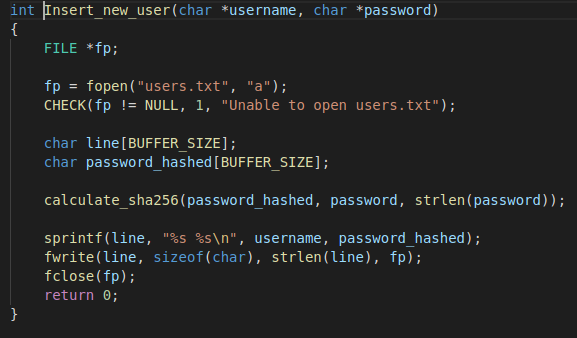
\includegraphics[width=\linewidth]{lognew.png}
  \caption{Inserare utilizator nou.}
  \label{fig:lognew}
\end{figure}

\subsection { Pastrarea credentialelor}
Credentialele se pastreaza intr-un fisier sub forma $username sha256_custom(password)$. 
Pentru a calcula sha256 pentru parola, am folosit o librarie si modificat-o astfel incat sa imi functioneze. \cite{ref_sha256}

%
% ---- Bibliography ----\
\bibliographystyle{splncs04}
%
\begin{thebibliography}{9}

\bibitem{ref_tcp1}
Tutorial tradus de Ionuţ Lucaşl , 4--6 \\
\url{https://profs.info.uaic.ro/busaco/teach/courses/net/docs/tcpip\_net-ro.pdf}


\bibitem{ref_rsa}
Wikipedia page pentru RSA , 4--6 \\
\url{https://ro.wikipedia.org/wiki/RSA}


\bibitem{ref_rsa}
Wikipedia page pentru RSA , 4--6 \\
\url{https://ro.wikipedia.org/wiki/RSA}


\bibitem{ref_sha256}
Sha256 library \\
\url{https://github.com/amosnier/sha-2}


\end{thebibliography}  


\end{document}
